%%%%%%%%%%%%%%%%%%%%%%%%%%%%%%%%%%%%%%%%%
% Short Sectioned Assignment
% LaTeX Template
% Version 1.0 (5/5/12)
%
% This template has been downloaded from:
% http://www.LaTeXTemplates.com
%
% Original author:
% Frits Wenneker (http://www.howtotex.com)
%
% License:
% CC BY-NC-SA 3.0 (http://creativecommons.org/licenses/by-nc-sa/3.0/)
%
%%%%%%%%%%%%%%%%%%%%%%%%%%%%%%%%%%%%%%%%%

%----------------------------------------------------------------------------------------
%	PACKAGES AND OTHER DOCUMENT CONFIGURATIONS
%----------------------------------------------------------------------------------------

\documentclass[paper=a4, fontsize=11pt]{scrartcl} % A4 paper and 11pt font size
\usepackage[section]{placeins}

\usepackage[T1]{fontenc} % Use 8-bit encoding that has 256 glyphs
%\usepackage{fourier} % Use the Adobe Utopia font for the document - comment this line to return to the LaTeX default
\usepackage[english]{babel} % English language/hyphenation
\usepackage{amsmath,amsfonts,amsthm} % Math packages
\usepackage{units}
\makeatletter
\AtBeginDocument{%
  \expandafter\renewcommand\expandafter\subsection\expandafter{%
    \expandafter\@fb@secFB\subsection
  }%
}
\makeatother
\usepackage{hyperref}
\usepackage{lipsum} % Used for inserting dummy 'Lorem ipsum' text into the template
\usepackage{caption}

\usepackage{sectsty} % Allows customizing section commands
\allsectionsfont{\centering \normalfont\scshape} % Make all sections centered, the default font and small caps
\usepackage{amsmath}
\usepackage{fancyhdr} % Custom headers and footers
\pagestyle{fancyplain} % Makes all pages in the document conform to the custom headers and footers
\fancyhead{} % No page header - if you want one, create it in the same way as the footers below
\fancyfoot[L]{} % Empty left footer
\fancyfoot[C]{} % Empty center footer
\fancyfoot[R]{\thepage} % Page numbering for right footer
\renewcommand{\headrulewidth}{0pt} % Remove header underlines
\renewcommand{\footrulewidth}{0pt} % Remove footer underlines
\setlength{\headheight}{13.6pt} % Customize the height of the header
\usepackage{subcaption}
\numberwithin{equation}{section} % Number equations within sections (i.e. 1.1, 1.2, 2.1, 2.2 instead of 1, 2, 3, 4)
\numberwithin{figure}{section} % Number figures within sections (i.e. 1.1, 1.2, 2.1, 2.2 instead of 1, 2, 3, 4)
\numberwithin{table}{section} % Number tables within sections (i.e. 1.1, 1.2, 2.1, 2.2 instead of 1, 2, 3, 4)
\usepackage{graphicx}
\setlength\parindent{0pt} % Removes all indentation from paragraphs - comment this line for an assignment with lots of text

%----------------------------------------------------------------------------------------
%	TITLE SECTION
%----------------------------------------------------------------------------------------

\newcommand{\horrule}[1]{\rule{\linewidth}{#1}} % Create horizontal rule command with 1 argument of height

\title{	
\normalfont \normalsize 
\textsc{Michigan State University} \\ [25pt] % Your university, school and/or department name(s)
\horrule{0.5pt} \\[0.4cm] % Thin top horizontal rule
\huge  Project 2 \\ % The assignment title
\horrule{2pt} \\[0.5cm] % Thick bottom horizontal rule
}

\author{Alex Dombos, Samuel Lipschutz, Charles Loelius} % Your name

\date{\normalsize 2/5/14} % Today's date or a custom date

\begin{document}

\maketitle % Print the title

%----------------------------------------------------------------------------------------
%	PROBLEM 1
%----------------------------------------------------------------------------------------
\section{Derivations}



\subsection{}

Outside the finite range $R_{n}$ of the nuclear potential, the wave function expressed in terms of partial waves is

\begin{equation*}
\psi(R,\theta)\overset{R>R_{n}}{\rightarrow}\frac{1}{kR}\sum_{L=0}^{\infty}\left(2L+1\right)i^{L}P_{L}\left(\textrm{cos}\left(\theta\right)\right)A_{L}\left[H_{L}^{-}\left(0,kR\right)-S_{L}H_{L}^{+}\left(0,kR\right)\right]
\end{equation*}

%\begin{equation*}
%e^{ikz}=\sum_{L=0}^{\infty}(2L+1)i^{L}P_{L}(\textrm{cos}(\theta))\frac{1}{kR}\frac{i}{2}\left[H_{L}^{-}(0,kR)-H_{L}^{+}(0,kR)\right]
%\end{equation*}

\noindent We also know that the asymptotic form of the wave function is comprised of an incoming plane wave (which is decomposed into partial waves) and outgoing spherical waves

\begin{align*}
\psi^{\textrm{asym}}(R,\theta)&=e^{ikz}+f(\theta)\frac{e^{ikR}}{R}\\
&=\sum_{L=0}^{\infty}(2L+1)i^{L}P_{L}(\textrm{cos}(\theta))\frac{1}{kR}\frac{i}{2}\left[H_{L}^{-}(0,kR)-H_{L}^{+}(0,kR)\right]+f(\theta)\frac{e^{ikR}}{R}\\
\end{align*}

\noindent Equating these two expressions gives

\tiny
\begin{align*}
\psi(R>R_{n},\theta)&=\psi^{\textrm{asym}}\\
\frac{1}{kR}\sum_{L=0}^{\infty}\left(2L+1\right)i^{L}P_{L}\left(\textrm{cos}\left(\theta\right)\right)A_{L}\left[H_{L}^{-}\left(0,kR\right)-S_{L}H_{L}^{+}\left(0,kR\right)\right]&=\sum_{L=0}^{\infty}(2L+1)i^{L}P_{L}(\textrm{cos}(\theta))\frac{1}{kR}\frac{i}{2}\left[H_{L}^{-}(0,kR)-H_{L}^{+}(0,kR)\right]+f(\theta)\frac{e^{ikR}}{R}\\
\left(kR\right)\left\{\frac{1}{kR}\sum_{L=0}^{\infty}\left(2L+1\right)i^{L}P_{L}\left(\textrm{cos}\left(\theta\right)\right)A_{L}\left[H_{L}^{-}\left(0,kR\right)-S_{L}H_{L}^{+}\left(0,kR\right)\right]\right\}&=\left(kR\right)\left\{\sum_{L=0}^{\infty}(2L+1)i^{L}P_{L}(\textrm{cos}(\theta))\frac{1}{kR}\frac{i}{2}\left[H_{L}^{-}(0,kR)-H_{L}^{+}(0,kR)\right]+f(\theta)\frac{e^{ikR}}{R}\right\}\\
\sum_{L=0}^{\infty}\left(2L+1\right)i^{L}P_{L}\left(\textrm{cos}\left(\theta\right)\right)A_{L}\left[H_{L}^{-}\left(0,kR\right)-S_{L}H_{L}^{+}\left(0,kR\right)\right]&=\sum_{L=0}^{\infty}(2L+1)i^{L}P_{L}(\textrm{cos}(\theta))\frac{i}{2}\left[H_{L}^{-}(0,kR)-H_{L}^{+}(0,kR)\right]+kf(\theta)e^{ikR}\\
\sum_{L=0}^{\infty}\left(2L+1\right)i^{L}P_{L}\left(\textrm{cos}\left(\theta\right)\right)A_{L}\left[i^{L}e^{-ikR}-S_{L}i^{-L}e^{ikR}\right]&=\sum_{L=0}^{\infty}(2L+1)i^{L}P_{L}(\textrm{cos}(\theta))\frac{i}{2}\left[i^{L}e^{-ikR}-S_{L}i^{-L}e^{ikR}\right]+kf(\theta)e^{ikR}\\
\end{align*}
\normalsize

\noindent The asymptotic forms of the Hankel functions were used in the last step. Now the terms with $e^{ikR}$ and $e^{-ikR}$ factors are collected together separately.

\scriptsize
\begin{equation*}
e^{ikR}\left[ \sum_{L=0}^{\infty}(2L+1)i^{L}P_{L}(\textrm{cos}(\theta)) \left\{A_{L}S_{L}i^{-L}-\frac{i}{2}i^{-L}\right\}+kf(\theta) \right]=e^{-ikR}\left[ \sum_{L=0}^{\infty}(2L+1)i^{L}P_{L}(\textrm{cos}(\theta)) \left\{A_{L}i^{L}-\frac{i}{2}i^{L}\right\} \right]
\end{equation*}
\normalsize

\noindent Since the expressions in the square brackets are independent of R, and $e^{\pm ikr}$ are linearly independent, the expressions in the square brackets must equal zero independently. Also, due to the orthogonality of the Legendre Polynomials, for the second expression in the square brackets to be zero for all L, then each term in the sum must be zero. This means $A_{L}=i/2$. % Consider a*cos(x) = b*sin(x). cos(x) and sin(x) are linearly independent. For this to be true for all x, then a and b must equal 0.

Using $A_{L}=i/2$ in the first term with the square brackets gives

\begin{align*}
&e^{ikR}\left[ \sum_{L=0}^{\infty}(2L+1)i^{L}P_{L}(\textrm{cos}(\theta)) \left\{A_{L}S_{L}i^{-L}-\frac{i}{2}i^{-L}\right\}+kf(\theta) \right]=0\\
&\Rightarrow \left[ \sum_{L=0}^{\infty}(2L+1)i^{L}P_{L}(\textrm{cos}(\theta)) \left\{\left(\frac{i}{2}\right)S_{L}i^{-L}-\frac{i}{2}i^{-L}\right\}+kf(\theta) \right]=0\\
&\Rightarrow \sum_{L=0}^{\infty}(2L+1)i^{L}P_{L}(\textrm{cos}(\theta))\left(\frac{i}{2}i^{-L}\right)(S_{L}-1) = -kf(\theta)\\
&\Rightarrow \left(\frac{i}{2}\right)\left(\frac{-1}{k}\right)\left(\frac{i}{i}\right)\sum_{L=0}^{\infty}(2L+1)P_{L}(\textrm{cos}(\theta))(S_{L}-1) = f(\theta)\\
&\Rightarrow f(\theta)=\frac{1}{2ik}\sum_{L=0}^{\infty}(2L+1)P_{L}(\textrm{cos}(\theta))(S_{L}-1)\\
\end{align*}

\subsection{}

The scattering amplitude can be written as

\begin{align*}
f(\theta)&=\frac{1}{2ik} \sum_{L=0}^{\infty} (2L+1)P_{L}(\textrm{cos}(\theta))(S_{L}-1)\\
&=\frac{1}{2ik} \sum_{L=0}^{\infty} (2L+1)P_{L}(\textrm{cos}(\theta))\left[ e^{2i\delta_{L}}-1\right]\\
&=\frac{1}{2ik} \sum_{L=0}^{\infty} (2L+1)P_{L}(\textrm{cos}(\theta))\left[ e^{i\delta_{L}}(e^{i\delta_{L}}-e^{-i\delta_{L}})\right]\\
&=\frac{1}{2ik} \sum_{L=0}^{\infty} (2L+1)P_{L}(\textrm{cos}(\theta))\left[ 2ie^{i\delta_{L}}\textrm{sin}(\delta_{L})\right]\\
&=\frac{1}{k} \sum_{L=0}^{\infty} (2L+1)P_{L}(\textrm{cos}(\theta))e^{i\delta_{L}}\textrm{sin}(\delta_{L})\\
\end{align*}

Using this, the total elastic cross section for neutrons is 

\footnotesize
\begin{align*}
\sigma_{\textrm{el}}&=\int |f(\theta)|^{2}d\Omega\\
&=\int_{0}^{2\pi} d\phi \int_{0}^{\pi} |f(\theta)|^{2} \textrm{sin}(\theta) d\theta\\
&=\int_{0}^{2\pi} d\phi \int_{0}^{\pi} \left[\frac{1}{k} \sum_{L'=0}^{\infty} (2L'+1)P_{L'}(\textrm{cos}(\theta))e^{i\delta_{L'}}\textrm{sin}(\delta_{L'})\right]^{*}\left[\frac{1}{k} \sum_{L=0}^{\infty} (2L+1)P_{L}(\textrm{cos}(\theta))e^{i\delta_{L}}\textrm{sin}(\delta_{L})\right]\textrm{sin}(\theta)d\theta\\
&=\frac{2\pi}{k^{2}}\sum_{L'=0}^{\infty}\sum_{L=0}^{\infty}(2L'+1)(2L+1)e^{-i\delta_{L'}}\textrm{sin}(\delta_{L'})e^{i\delta_{L}}\textrm{sin}(\delta_{L})\left[\int_{0}^{\pi}P_{L'}(\textrm{cos}(\theta))P_{L}(\textrm{cos}(\theta))\textrm{sin}(\theta)d\theta \right]\\
&=\frac{2\pi}{k^{2}}\sum_{L'=0}^{\infty}\sum_{L=0}^{\infty}(2L'+1)(2L+1)e^{-i\delta_{L'}}\textrm{sin}(\delta_{L'})e^{i\delta_{L}}\textrm{sin}(\delta_{L})\left[\frac{2}{2L+1}\delta_{LL'} \right]\\
&=\frac{2\pi}{k^{2}}\sum_{L'=0}^{\infty}(2L'+1)(2L'+1)e^{-i\delta_{L'}}\textrm{sin}(\delta_{L'})e^{i\delta_{L'}}\textrm{sin}(\delta_{L'})\frac{2}{2L'+1}\\
&=\frac{4\pi}{k^{2}}\sum_{L'=0}^{\infty}(2L'+1)\textrm{sin}^{2}(\delta_{L'})
\end{align*}
\normalsize

Relabeling $L'$ to $L$ gives the desired result

\begin{equation*}
\sigma_{\textrm{el}}=\frac{4\pi}{k^{2}}\sum_{L=0}^{\infty}(2L+1)\textrm{sin}^{2}(\delta_{L})
\end{equation*}

\subsection{}

If considering proton scattering instead of neutron scattering, the Coulomb interaction must be included in the calculation of the elastic scattering phase shift. The Coulomb interaction is included by modifying the asymptotic forms of the Hankel functions, $H_{L}^{\pm}$. The asymptotic form of the Hankel functions are now $H_{L}^{\pm} \left( \eta, \rho \right) \sim e^{i\Theta}$ where $\Theta= \left[ \rho - L \frac{\pi}{2} + \sigma_{L}\left( \eta \right) - \eta \textrm{ln} \left(2 \rho \right) \right]$ and $\sigma_{L} \left( \eta \right) = \textrm{arg}\Gamma\left(1+L+i\eta \right)$ is the Coulomb phase shift. The infinite range of the Coulomb potential is reflected in the term $\textrm{ln} \left(2 \rho \right)$, which never goes away for large $\rho$.

\section{Target Selection}

In this case, we consider the setup to be a target of stable $^{58}$Ni, in its ground state. We thereby find that we have quantum numbers in the entrance partition corresponding to (assuming neutron/proton scattering):\\
\begin{center}
\begin{table}[h!]
\captionsetup{font=large}
\caption{Table of Quantum Values}
\centering
\vspace{3 mm}
\begin{tabular}{|c|c|}

Quantum Number & Value \\
Mass partition x & T=58,P=1\\
Charge & 28 \\
Spin & 0\\
Parity & +


\end{tabular}
\end{table}
\end{center}



\section{Pointlike and Structured Coulomb Scattering}

We would expect, in the absence of any nuclear forces, and for a point like nucleus, that that the proton would have a pure Rutherford cross section.Upon taking into account the finite size of the target, we recognize that there is a perturbation in the distribution of charge, so that the electric potential will switch from a $\frac{1}{r}$ term to a linear term proportional to $r$. We expect that this should mean that at energies high enough to probe the structure of the proton-i.e. those that can overcome the Coulomb potential to have a reasonably large wavefunction in the vicinity of the proton- there ought to be an increased cross section in the forward direction. \\

We compare this below to four graphs of the Coulomb potential, one pointlike and one with spatial extent, with energies of .1 MeV and 50 MeV.\\

 \begin{figure}[hbt]
        \centering
        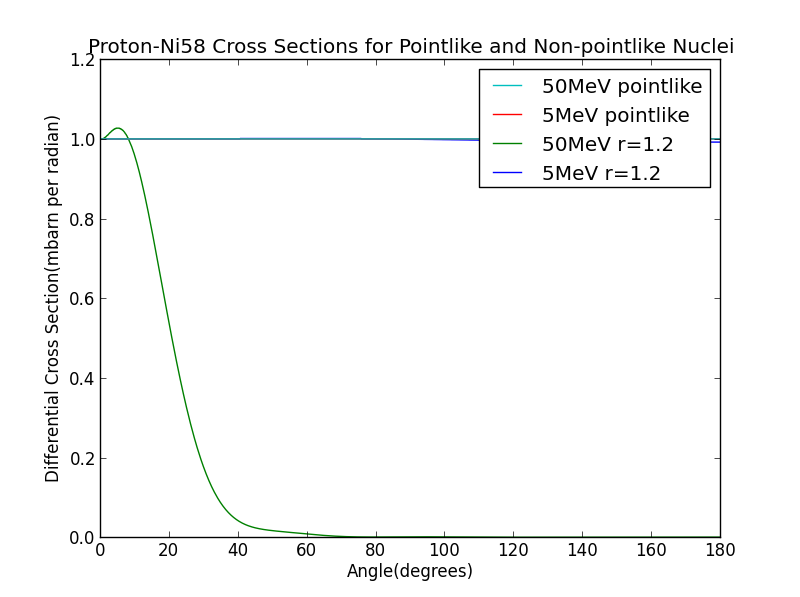
\includegraphics[width=.6\textwidth]{Pointcompare}
        \caption{Comparison of Pointlike (top) and Extended (bottom) Coulomb Cross Sections }
\end{figure}

We see that this is exactly what was anticipated, that the pointlike Coulomb scattering is indentical to the Rutherford cross section, whereas the case where the target (Nickel-58) has a radial extent shows no structure for low-energy projectiles but has the expected forward peaking for high energy. \\

\section{Proton-Nickel Analysis}
\subsection{Differential Cross Sections}

Here we examine the cross sections for the case of proton scattering on $^{58}$Ni with an optitcal potential paramaterized into volume, surface and spin-orbit components.  Below in figure 4.1 we have the full potential (left) and only the real terms included (right).  In all cases we see the cross section (plotted vs. the Rutherford cross section) approach 1 at 0 degrees.  This is expected as the Coulomb component diverges strongly at 0 degrees and should dominate.  For the case of 5 MeV protons we see only small deviations away from the Rutherford cross section, since at this energy the Coulomb barrier is shielding the details of the optical potential.   


 \begin{figure}[hbt]
        \centering
        \begin{subfigure}[b!]{0.35\textwidth}
                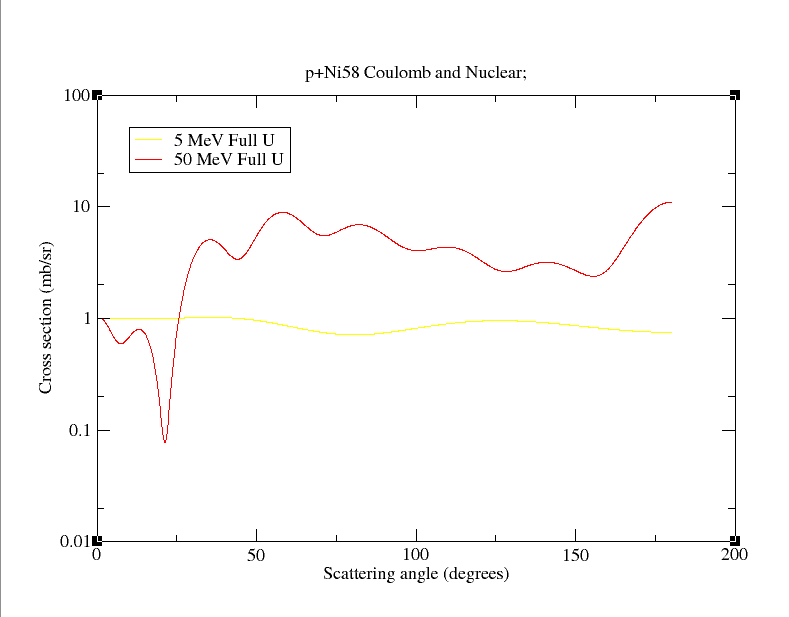
\includegraphics[width=\textwidth]{FullUComp.PNG}
        \end{subfigure}%
        ~ %add desired spacing between images, e. g. ~, \quad, \qquad etc.
          %(or a blank line to force the subfigure onto a new line)
\quad
        \begin{subfigure}[b!]{0.35\textwidth}
                \includegraphics[width=\textwidth]{NoImuComparison.PNG}
        \end{subfigure}

        \caption{Differential Cross Sections for Proton Interactions}
\end{figure}

Below in figure 4.2 we have a comparision of the cross section with and without the imaginary part of the potential.  Seen in both the 5 MeV and 50 MeV cases the overall strength is reduced for the potential containing imaginary components.  This is expected as the loss of flux created by the imgainary potential should lower the probability of elastic scatterings.  

 \begin{figure}[hbt]
        \centering
        \begin{subfigure}[b!]{0.35\textwidth}
                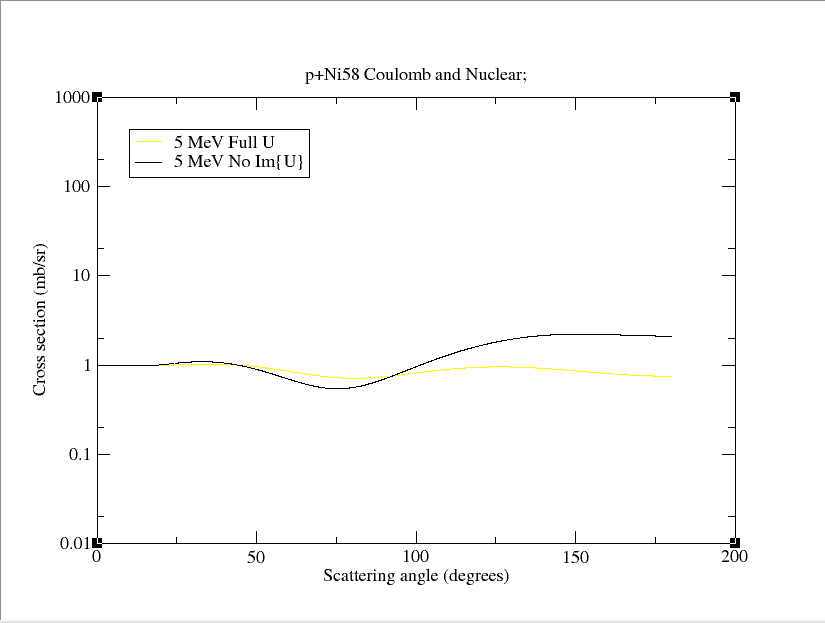
\includegraphics[width=\textwidth]{5MeVUandNoUComp.PNG}
        \end{subfigure}%
        ~ %add desired spacing between images, e. g. ~, \quad, \qquad etc.
          %(or a blank line to force the subfigure onto a new line)
\quad
        \begin{subfigure}[b!]{0.35\textwidth}
                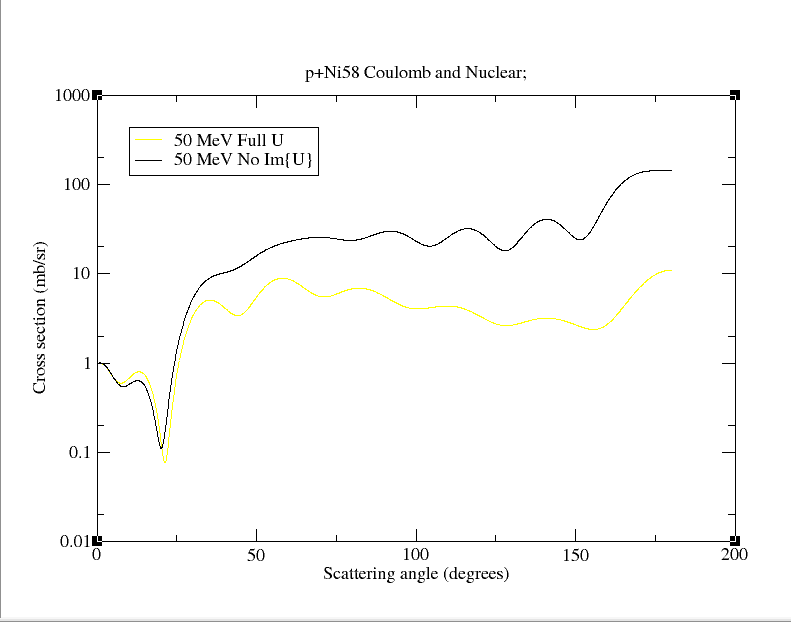
\includegraphics[width=\textwidth]{50MeVnoUandUcomp.PNG}
        \end{subfigure}

        \caption{Differential Cross Sections for Proton Interactions}
\end{figure}
 

\subsection{S-Matrix Components}
Below in figure 4.3 we have the modulus of the S-Matrix vs. total J.  As one expects, the case where there is no imaginary component of the potential all the values are 1.  Without a loss of flux the S-Matrix must be unitary.  In the opposing case there is strong deviation from 1 for the lower partial waves.  Further it is seen that the values quickly converge around $L=10$, and despite this we have calculated all the way out to $L=100$.
\begin{figure}[hbt]
        \centering
	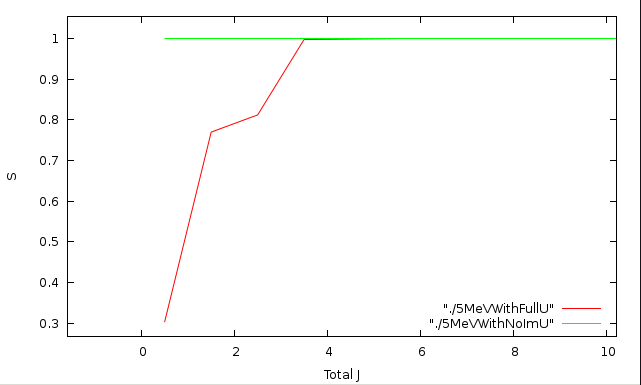
\includegraphics[width=.4\textwidth]{SMatrixV_J.PNG}
 \caption{Modulus of the S-Matrix values as a function of J}	
\end{figure}


\subsection{Increased Radii and Diffusiveness}

Below in figure 4.4 the cross sections for different radii and diffuseness parameters are compared.  In both cases the values were increased by a factor of 1.5 in all the terms of the potential (volume, surface and spin-orbit).  On the left is the increased radius case.  Here the 5 MeV protons move farther from the pure Rutherford case as the extent of the nuclear interaction has been increased.  We see this also in the 50 MeV case where the overall trend tends to be amplified.  On right we have the increased diffuseness case.  Here we again see more deviation from pure Rutherford for the 5 MeV protons, but we also see a decrease in the backward angles.  If we had decreased the diffuseness, making the potential more like a delta funcion, then we would expect there to be an increase in the backward angles.  As it becomes more diffuse there are more ways to scatter to foward angles, causing a decrease in backward angles.

 \begin{figure}[hbt]
        \centering
        \begin{subfigure}[b!]{0.35\textwidth}
                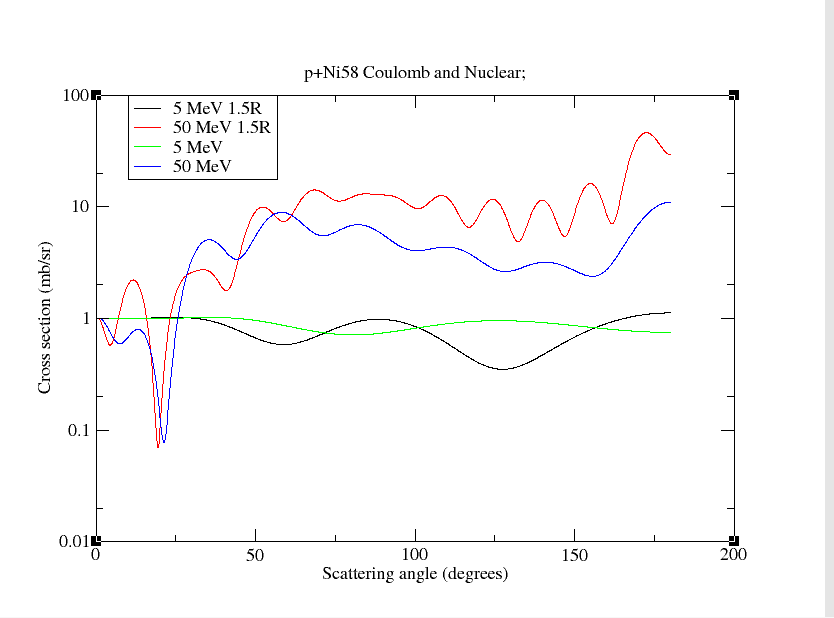
\includegraphics[width=\textwidth]{ChangedRadius.PNG}
        \end{subfigure}%
        ~ %add desired spacing between images, e. g. ~, \quad, \qquad etc.
          %(or a blank line to force the subfigure onto a new line)
\quad
        \begin{subfigure}[b!]{0.35\textwidth}
                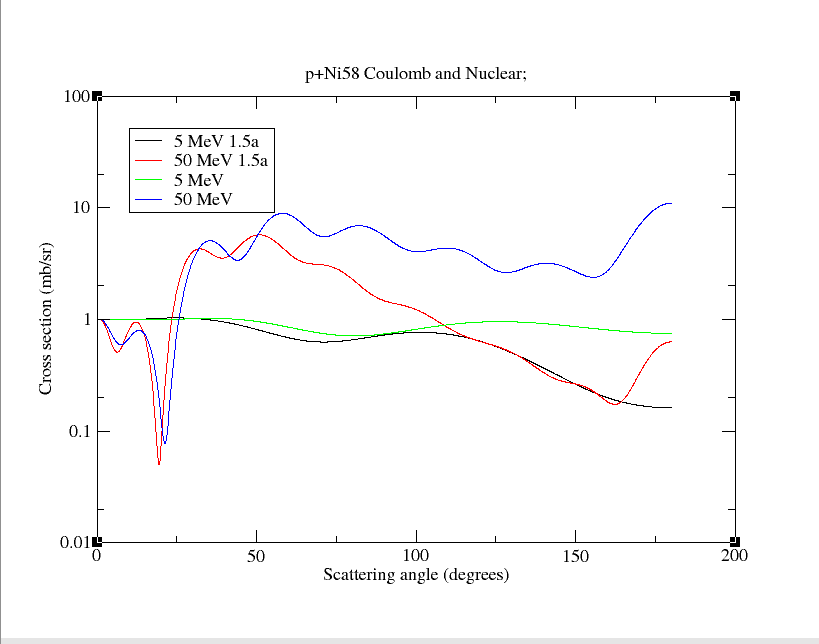
\includegraphics[width=\textwidth]{ChangedDiff.PNG}
        \end{subfigure}

        \caption{Comparison of increased Radii (left) and diffuseness (right) to original potential values}
\end{figure}


\section{Neutron-Nickel Analysis}
\subsection{Differential Cross Sections}
We then consider the previous analysis using a similar potential model for the nuclear optical potential, but setting the charge of the projectile to 0, and changing the optical potential to be for n-scattering as found in Reference 2 below. The results of this are plotted below.\\


 \begin{figure}[hbt]
        \centering
	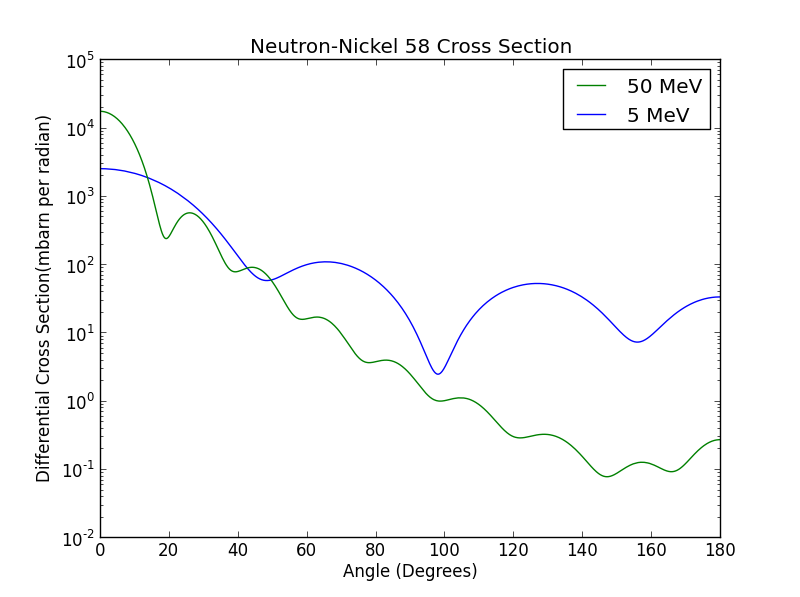
\includegraphics[width=.6\textwidth]{CrossSectionsNEns}
        \caption{Differential Cross Sections for Neutron Interactions}
\end{figure}

We can see in this case that the distributions are sharply peaked near zero, with the major difference being in the extreme sharpness of the 50 MeV compared to a somewhat  broader peak for the 5 MeV. This makes sense because the 50 MeV neutron has a larger energy compared to the optical potential and so is less affected. However, the 5 MeV neutron  is likely to interact more with the optical potential. This explains the broader scattering. We might expect something similar as energy decreases and the optical potential causes further interactions. However, this must be reconciled with an expected decrease in flux caused by increase interactions with the imaginary potential.We note that in this instance the cross sections are not being compared to the infinite rutherford and so in principle has a smaller forward cross section than the proton scattering. \\

\subsection{Increased Diffuseness}

In this case, I have set the diffuseness parameter to be times larger than in the standard parameter found in the previous optical potential. This results in a cross section as follows (for 50 MeV):\\
\begin{figure}[!hbt]
\centering
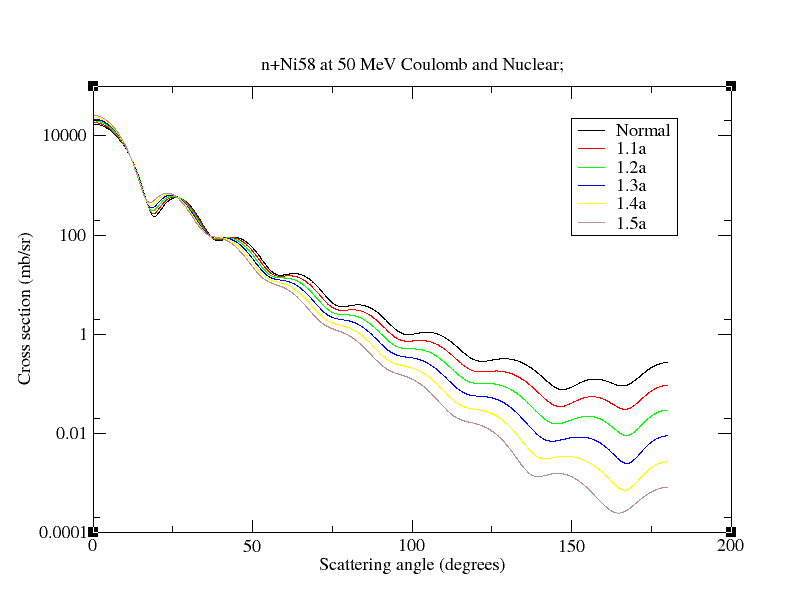
\includegraphics[width=.6\textwidth]{NeutronDiff.png}
\end{figure}

We see in this case that the increased diffusiveness reduces substantially the amount of backwards scattering, as we would expect. Naively, this is akin to replacing the Rutherford model of the nucleus with something ore akin to the "plum pudding model", and so diminishing its concentrated strength which allows for backwards scattering. Of course, this interpretation is only very rough, as of course the coulomb interaction is irrelevant in this instance, but the general picture of a more or less pointlike source being more or less capable of deflecting particles at large angles is still a useful way to think about this situation.




\subsection{Increased Radius}

In this case we consider a radius parameter in the optical potential to be larger than in the potential defined above. This has the effect of increasing the range over which the potential is strong, and so increases the overall effect of the potential, leaving a larger relative amount of the cross section over which to be scattered. This leads to an increase in larger angle scattering since there is a wider range over which these angles can be reached. However, it also increases the surface area and volume, which means that there is an increased probability for absorption through the imaginary potential and so could contribute to an overall smaller cross section. In addition we see a change in the oscillatory behaviour of the cross section. We can understand this in a naive model if we consider the simple case of a finite square well as an exceptionally rough approximation to the infinite but quickly vanishing optical potential. In this case, recognizing that the incoming particle has its own De Broigle wavelength, we would expect a certain diffraction patern. As the radius of the well changes, it will shift the transmission and reflection probabilities, thus changing the overall diffraction patern. While this is a simple model, it nonetheless this does explain some of the results, for example the far more quickly oscillating behaviour of the 50 MeV cross section, and the somewhat linear slight phase shift there as r increases(most clearly seen in  the ~20 radians regime. It also explains the far from linear phase shifting and amplitude modifying behaviour in the 5MeV case, as in this case the De Broigle wavelength is much larger, and so we would expect it to be closer to the radius of the potential well. Hence it  would be anticpated to be affected more by the change in radius of the potential well. 


\begin{figure}[hbt]
\centering
\begin{subfigure}[b!]{.45\textwidth}
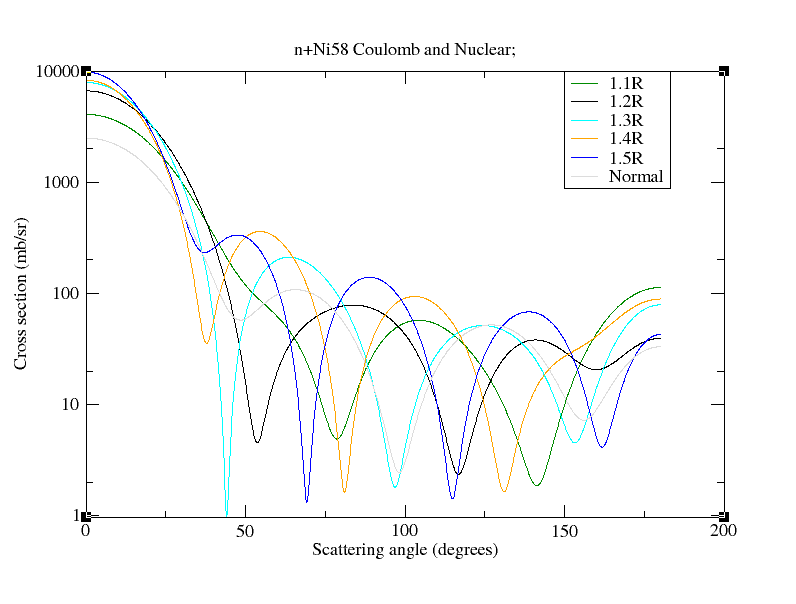
\includegraphics[width=\textwidth]{NeutronRad5.png}
\caption{5 MeV}
\end{subfigure}
\quad
\begin{subfigure}[b!]{.45\textwidth}
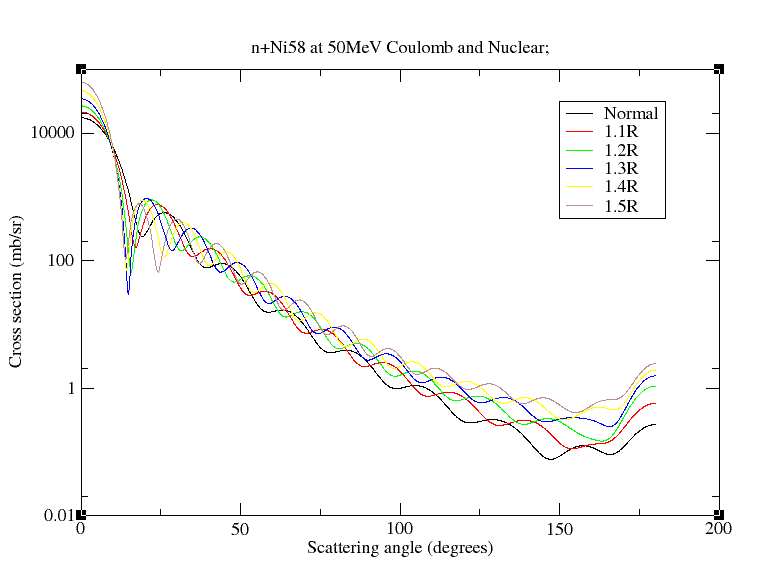
\includegraphics[width=\textwidth]{NeutronRad50.png}
\caption{50 MeV}
\end{subfigure}
\caption{Cross Sections For Varied Radii}
\end{figure}

\subsection{Different Strength of Imaginary Potentials}

We then ought to anticipate a difference in the total cross sections and so the elastic differential cross sections of the potential, and so a strong imaginary potential(in this case multiplied by ten from the above) ought to have a much smaller cross section than that of the weak potential (in this case wth the strength of the imaginary potentials divided by ten).

These are plotted below:

 \begin{figure}[hbt!]
        \centering
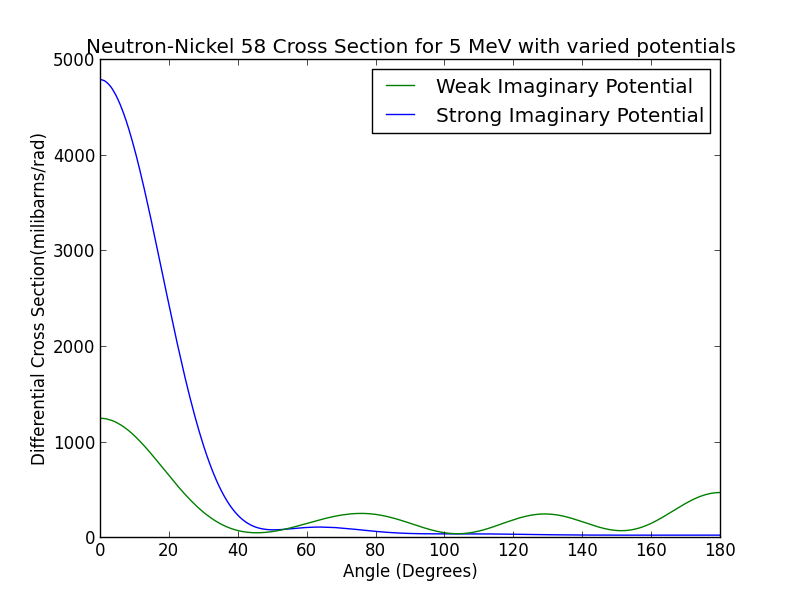
\includegraphics[width=.6\textwidth]{Imcross}
        \caption{Differential Cross Sections for Neutron-Ni58 with Varying Imaginary Potentials}
\end{figure}
We note that in this instance we don't seem to have the same agreement expected, as it would appear that there is a larger cross section with the strong imaginary potential. However, we must recall that the angular integrated cross section picks up a factor of $\sin\theta$, and so the total cross section picks up very little of the forward cross section. For a better understanding instead we should look at the modulus of the S matrices for different L states, which will show the overall absorption. These are plotted below:\\


 \begin{figure}[hbt!]
        \centering
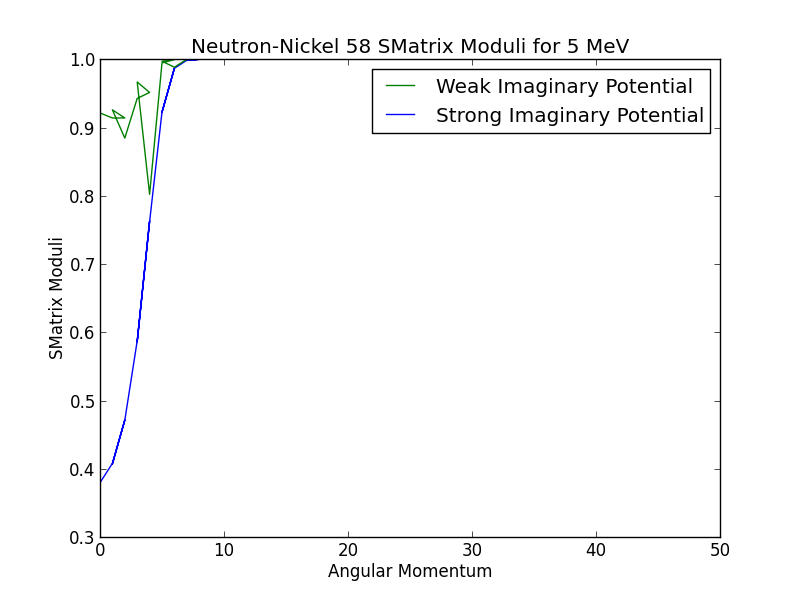
\includegraphics[width=.6\textwidth]{NeutronSms}

        \caption{Moduli of S-Matrix for Neutron-Ni58 with Varying Imaginary Potentials}
\end{figure}
\FloatBarrier
\vspace{ 5mm}
H
ere we see clearly that especially at low angular momenta the strong imagnary potential starts with a much smaller S matrix than that of the weak potential, and only slowly converges to 1 with a large L. \\

Finally we compare to the total cross sections, shown in the table below(Where the weak imaginary has no imaginary potential, and the strong has each of the imaginary strengths as 20.):\\
\begin{table}[hbt!]
\centering
\begin{tabular} {|c|c|c|c|}
Energy(MeV) & Imaginary Potential & Elastic Cross Section(mbarns) & Total Cross Section(mbarns)\\
50 & Weak & 3431 & 3431\\
50 & Strong & 1908 & 3973\\
5 & Weak & 2512 & 2512 \\
5 & Strong & 2420 & 4838 \end{tabular}\caption{Cross Sections for Varied Energies and Potentials}\end{table}

We can see clearly that while the change in energy can obscure the importance of the strong and weak potentials, the fact that the strong potential leads to about half of the total cross section being absorbed is very clear, be it for 50 or 5 MeV. This is as might be anticipated. However, the fact that the potential was scaled so the volume and surface terms were equally as important obscures some of the more complicated features between energy and absorption that can be noticed in the optical potential models like those linked to, since increased energy will lead to more influence of the volume term than the surface term, and of course the opposite holds as well. 

\section{Total Cross Sections}

We return to the 5 and 50 MeV neutron-Ni58 scattering previously examined, noting that in the output files generated there is in fort.40 a description of the cross sections. We plot the results in the table below:\\

\begin{table}[hbt!]
\centering
\begin{tabular}{|c|c|c|c|}
Energy (MeV) & Reaction  (mbarn) & Elastic (mbarn)& Total (mbarn)\\
5 & 2262 & 1802 & 4064 \\
50 & 1548 &1889 & 3437 
\end{tabular}
\caption{Table of Cross Sections}
\end{table}

And in this we see that the high-energy neutron has a lower overall cross section, primarily driven by an increased lack of reactions as the potential is unable to affect the high energy neutron much.
\section{ Potential References}

\subsection{Protons} A. J. Koning, J. P. Delaroche, Nucl. Phys. A713, 231 (2003). Using the Reference Input Parameter Library, this corresponds to the OMP index of 4421. The specific URL is \url{https://www-nds.iaea.org/cgi-bin/ripl_om_param.pl?Z=28&A=58&ID=4421&E1=0.1&E2=150}.
\subsection{Neutrons}A. J. Koning, J. P. Delaroche, Nucl. Phys. A713, 231 (2003). Using the Reference Input Parameter Library, this corresponds to the OMP index of 4117. The specific URL is \url{https://www-nds.iaea.org/cgi-bin/ripl_om_param.pl?Z=28&A=58&ID=1417&E1=0.1&E2=150}.


\end{document}
